%%%%%%%%%%%%%%%%%%%%%%%%%%%%%%%%%%%%%%%%%%%%%%%%%%%%%%%%%%%%%%%%%%%%%%%
\section{Lecture 12 (Martin Kalck); The Cox Category, I: Definition}\label{lec:12-DCox-definition}
As we saw in one of the introductory lectures, Beilinson gave a very concrete description of the derived category of $\PP^n$~\cite{beilinson}.  Recall the
\defi{Beilinson collection} of line bundles $\cO_{\PP^n}(-n), \ldots,
\cO_{\PP^n}(-1), \cO_{\PP^n}$.  And the fact that the Beilinson collection is a full, strong, exceptional collection means that every sheaf on $\PP^n$ can be represented, in an essentially unique way, as a complex whose terms are sums of these line bundles.

\begin{thm}\label{thm:BeilinsonFSEC}
The Beilinson collection of line bundles on $\PP^n$ is a full, strong exceptional collection.
\end{thm}


\begin{thm}\label{thm:UniquenessAndFSEC}
    For every sheaf $\mathcal F$ on $\PP^n$, there is a (unique up to homotopy) complex $F$ which is quasisomorphic to $\mathcal F$ and where $F_i = \oplus_{j=0}^n \cO(-j)^{m_{ij}}$.
\end{thm}

Some well-known toric varieties satisfy an analogue of Beilinson's theorem.

\begin{example}
    The Beilinson collection for $\PP^1$ consists of the line bundles of degrees $-1$ and $0$.   On $\PP^1\times \PP^1$, the bundles $\cO_{\PP^1\times \PP^1}(-1,-1),\cO_{\PP^1\times \PP^1}(-1,0), \cO_{\PP^1\times \PP^1}(0,-1),\cO_{\PP^1\times \PP^1}$ form a full, strong exceptional collection.  Note that the degrees that arise are the products of the degrees from the Beilinson collection of the factors.  A variant of Theorem~\ref{thm:UniquenessAndFSEC} thus holds for sheaves on $\PP^1\times \PP^1$.

    A similar result holds for any product $\PP^n\times \PP^m$.  In this case, the degrees that should up at $\cO(-i,-j)$ where $-n \leq -i \leq 0$ and $-m \leq -j \leq 0$.  In fact, a similar result holds for multifactor products like $\PP^a\times \PP^b\times \PP^c\times \PP^d$.

    The proofs of all of these cases follow fairly easily from Beilinson's original work.  This is for the following reasons:
    \begin{enumerate}
        \item Exceptionality is a simple calculation.
        \item Fullness follows easily from having a resolution of the diagonal like Beilinson's.
        \item If $F$ is Beilinson's resolution of the diagonal for $\PP^n$ and $G$ is Beilinson's resolution of the diagonal for $\PP^m$ then $F\boxtimes G$ is a resolution of the diagonal for $\PP^n\times \PP^m.$
    \end{enumerate}

    For instance, in the case of $\PP^1\times \PP^1$ in more detail.  The fact that
    \[
    \cO_{\PP^1\times \PP^1}(-1,-1),\cO_{\PP^1\times \PP^1}(-1,0), \cO_{\PP^1\times \PP^1}(0,-1),\cO_{\PP^1\times \PP^1}
    \]form a strong exceptional collection is a simple cohomology computation.  For fullness, we start with the fact that
    \[
    \cO_{(\PP^1)^2} \gets \cO_{(\PP^1)^2}(-1,-1)\gets 0
    \]
     is a resolution of $\Delta_{\PP^1} \subseteq (\PP^1)^2$.  Taking the box product of this complex with itself yields a resolution of $\Delta_{(\PP^1)^2} \subseteq (\PP^1)^4$:
     \[
    \cO_{(\PP^1)^4} \gets
    \begin{matrix}
      \cO_{(\PP^1)^4}(-1,0,-1,0)\\
      \oplus
      \cO_{(\PP^1)^4}(0,-1,0,-1)
    \end{matrix}
    \gets
     \cO_{(\PP^1)^4}(-1,-1,-1,-1) \gets 0.
     \]
     Applying the Fourier--Mukai transform trick, similar to what we saw in Lecture 2 and in the proof of Conjecture~\ref{conj:bondal}, will show fullness.
\end{example}



Some of the other classical examples of smooth projective toric varieties also satisfy an analogue of Beilinson's theorem.
\begin{example}
Let $X$ be the Hirzebruch surface of type $3$, as introduced in Example~\ref{ex:Hirzebruch}.  Then $\cO_{X}(-1,-1),\cO_{X}(-1,0), \cO_{X}(0,-1),\cO_{X}$
form a full, strong exceptional collection.  The same result holds for a Hirzebruch surface of any type.  For those who are curious: this is a special case of Orlov's semi-orthogonal decomposition result for projective bundles.\daniel{add citation}
\end{example}

A natural question then is to ask:  which smooth, projective toric varieties satisfy an analogue of Beilnson's theorem?  In 1997, King conjectured that the answer was ``all of them''.

\begin{conj}[King, 1997]
    Every smooth, projective toric variety has a full, strong exceptional collection of line bundles.
\end{conj}

This turned out to be
false.  Hille-Perling gave the first counterexamples, and followup work of Michalek and Efimov showed counterexamples for fairly simple varieties, and showed that the conjecture could not be salvaged by restricting, for instance, to Fano toric varieties
~\cites{hille-perling, michalek11, efimov}.

Nevertheless, King's Conjecture
continued to inspire work on exceptional collections for toric
varieties, and there is a huge literature in this vein:
~\cites{altmann-immaculate,
BFK_GIT,BallardEtAl2019ArithmeticToric,BallardEtAl2019ToricFrobenius,BallardEtAl2018arxivDerivedCategories,bernardi-tirabassi,borisov-hua,borisov-orlov-equivariant,borisov-wang,costa-miro-roig04,costa-miro-roig10,costa-miro-roig2,dey-lason-michalek,Jerby1,Jerby2,Jerby3,kawamataI,kawamataII,lason-michalek,ohkawa2013frobenius,prabhu-naik,sanchez2023derived,Uehara},
\emph{inter alia}.  The closest result to King's Conjecture was probably Kawamata's theorem, which proved a weakening the conjecture by dropping the line bundle requirement and removing the strongness condition~\cite{kawamataI}.  While this is a major result, the contrast with Beilinson's theorem is pretty stark: while Theorem~\ref{thm:UniquenessAndFSEC} yields unique representations of any sheaf in terms of well-known building blocks (the line bundles in the Beilinson collection), the representations from Kawamata's would fail to be unique, and they would be in terms of building blocks that we don't understand whatsoever.  Notably: it is open question whether the objects in Kawamata's collection are sheaves or whether they will necessarily involve compelxes of sheaves.

Over the remaining lectures, we will develop and prove an alternative
realization of King’s Conjecture.  (The king is dead, long live the king!)
The basic idea originates from three observations:
\begin{enumerate}
    \item Several distinct toric varieties can have the same Cox ring.
    \item  The Hanlon-Hicks-Lazarev Theorem shows that the analogue of Beilinson's resolution of the diagonal is uniform for all toric varieties with the same Cox ring.
    \item  The Bondal-Thomsen collection--which is also uniform for all toric varieties with the same Cox ring--is an excellent analogue of the Beilinson in many ways.
\end{enumerate}
The picture that emerges is the following:
\begin{center}
\begin{tabular}{c|c}
    $\PP^n$ & Smooth, projective toric variety \\ \hline
Beilinson collection   &  Bondal-Thomsen collection\\
Beilinson resolution of diagonal & HHL resolution of diagonal\\
Theorem~\ref{thm:BeilinsonFSEC} (King's Conjecture for $\PP^n$)    &  {\bf Revised King's Conjecture}
\end{tabular}
\end{center}
Note that the Bondal-Thomsen collection and the HHL resolution depend only on the Cox ring.  This suggests that the ``right'' analogue of Theorem~\ref{thm:BeilinsonFSEC}, i.e. the ``right'' version of King's Conjecture, should perhaps depend only on the Cox ring.  In other words, maybe a revised King's Conjecture will involve a category that combines the sheaves from all of the toric varieties with the same Cox ring.

This only raises another question:  if $X$ and $X'$ are two toric varieties with the same Cox ring, how do ``combine'' their derived categories?



More specifically, in Section 5.1, we saw that a multigraded polynomial ring $S$ determines a finite set of simplicial toric varieties $X_1, X_2, \dots, X_r$ each of which has a corresponding stack $\sX_1, \sX_2, \dots, \sX_r$.
How can we combine their derived categories?  That is to say: we want to define a single category--which we refer to
 as the \defi{Cox category}, and denote by $D_{\Cox}(X)$ or $D_{\Cox}(S)$--that combines the study of modules on these $\sX_i$ {\em simultaneously}.
The theorem we are driving for is:

\begin{thm}[Revised King's Conjecture]\label{thm:main1}
If $X$ is a projective toric variety with Cox ring $S$, then the Bondal--Thomsen collection, under a natural ordering, forms a full strong exceptional collection of line bundles for $D_{\Cox}(S)$.
\end{thm}

This should be viewed as a vague statement for the moment, as we have not defined $D_{\Cox}(S)$ precisely, nor have we have identified the Bondal--Thomsen collection as a subset of the Cox category.  But it gives a sense of where we are going: for toric varieties, the Bondal--Thomsen collection and the resolution of the diagonal only depend on the Cox ring.  And Theorem~\ref{thm:main1} is a revised King's Conjecture, and an extension of Theorem~\ref{thm:BeilinsonFSEC}, that also only depends on the Cox ring.

We now aim to make the theorem precise.
\begin{lemma}\label{lem:TildeX}
    There exists a smooth, toric stack $\widetilde{\sX}$ that admits proper birational maps $\pi_i\colon \widetilde{\sX} \to \sX_i$ for all $i=1,2,\dots,r$.
\end{lemma}
\begin{proof}
    At the level of varieties, this would be very standard as one could just take a simplicial refinement of the fans of each of the $X_i$.  Extending that proof to toric stacks requires working with additional notation of toric stacks, but there are very few new ideas and so we omit the proof.  See \cite{king}*{\S 3.1} for details.
\end{proof}

A standard fact \cite{king}*{Lemma 3.7} is that the (derived) pullback $\pi_i^*$ from $D(\sX_i)$ to $D(\widetilde{\sX})$ is fully faithful.\footnote{Because we are focused on derived categories, every time we write $\pi_i^*$ we should really be using the derived functor $L\pi_i^*$.  However, since we focus almost entirely on the pullbacks of line bundles, $L\pi_i^*$ and $\pi_i^*$ will coincide.  We will thus abuse notation and write $\pi_i^*$ throughout.}  Thus, $\pi_i^*$ essentially embeds the derived category of $\sX_i$ into the derived category of $\widetilde{\sX}$.
This provides a way to ``combine'' $D(\sX_1), D(\sX_2), \cdots, D(\sX_r)$: we can take the span of these categories inside of the ambient category $D(\widetilde{\sX})$.

\begin{defn}\label{defn:CoxCategory}
We define the Cox category of $S$, denoted $D_{\Cox}(S)$ as follows.  Since each pullback functor $\pi_i^*$ is fully faithful, $\pi_i^* D(\sX_i)$ is like a perfect copy of $D(\sX_i)$ that lives in $D(\widetilde{\sX})$.
We define $D_{\Cox}(S)$ as the subcategory of $D(\widetilde{\sX})$ generated\footnote{By ``generated'' we mean the smallest triangulated category containing these objects and that is closed under taking summands and extensions.} by $\pi_1^*D(\sX_1), \pi_2^* D(\sX_2), \dots, \pi_r^* D(\sX_r)$. In other words, $D_{\Cox}(S)$ is like the category generated by (the pullbacks of) all sheaves from all of the $\sX_i$.
\end{defn}
It is easy to check that the definition of $D_{\Cox}(S)$
does not depend upon the choice of $\widetilde{\sX}$ from Lemma~\ref{lem:TildeX}; see \cite{king}*{Corollary 3.9}.

 But these copies overlap.
\begin{example}
   For any $1\leq i \leq r$ consider the structure sheaf $\cO_{\sX_i}$.  We have $\pi_i^*\cO_{\sX_i} = \cO_{\tsX}$.  Thus $\cO_{\tsX}$ lies in the intersection of the copy of each $D(\sX_i)$.
\end{example}

%Similarly, since the $\sX_i$ are all birational, the algebraic torus in each $\sX_i$ and in $\widetilde{\sX}$ are naturally identified with one another.  If we let $e_i$ denote the identity point in that torus in $\sX_i$ and $\widetilde{e}$ be the identity point in $\widetilde{\sX}$, then $\pi_i^* \cO_{e_i} = \cO_{\widetilde{e}}$ for all $i$.  So again, we see that $\cO_{\widetilde{e}}$ lies in the intersection of the copy of $ D(\sX_i)$ for each $i$.

We can thus think of $D_{\Cox}(S)$ as ``gluing'' the various $D(\sX_i)$ together.  See Figure~\ref{fig:venn_diagram}.  The main results we will see ahead show that $D_{\Cox}(S)$ has nicer properties than any of the individual $D(\sX_i)$, in a manner that is (metaphorically at least) akin to how a projective variety can have nicer properties than its various affine patches.

\begin{figure}[htbp]
\centering
\begin{tikzpicture}[scale=1.0]

    % Define the ovals (ellipses) with rotation for a symmetrical layout
    % Oval 1: Top
\draw[thick] (0, 0.4) ellipse (4.8cm and 3.2cm);

    \node[ellipse, draw, minimum width=4cm, minimum height=2.5cm, rotate=90]
        (A) at (0, 1.2) {};

    % Oval 2: Bottom Left
    \node[ellipse, draw, minimum width=4cm, minimum height=2.5cm, rotate=150]
        (B) at (-0.95, -0.4) {};

    % Oval 3: Bottom Right
    \node[ellipse, draw, minimum width=4cm, minimum height=2.5cm, rotate=30]
        (C) at (0.95, -0.4) {};

    % Outer labels for the sets
    \node[below left, xshift=-34mm] at (-1,2.5) {$D(\widetilde{\mathcal X})$};
    \node[above, yshift=15mm] at (A.north) {$D(\mathcal{X}_1)$};
    \node[below left, xshift=-34mm] at (B.south west) {$D(\mathcal{X}_2)$};
    \node[below right, xshift=-3mm] at (C.south east) {$D(\mathcal{X}_3)$};

    % Center intersection point and its label
    \filldraw (0, 0.15) circle (2pt) node[below, yshift=-2mm] {$\mathcal{O}_{\widetilde{\mathcal{X}}}$};

\end{tikzpicture}
\caption{The Cox category is built by embedding the categories of the $\sX_i$ into the ambient category $D(\tsX)$.  These copies overlap, and so the Cox category is like a gluing of the sheaves on the $\sX_i$.}
\label{fig:venn_diagram}
\end{figure}

% How do the copies of $D(\sX_i)$ in $D_{\Cox}$ relate to one another?
% The graphs of the birational maps $\sX_i \dashrightarrow \sX_j$ induce
% Fourier--Mukai transforms  $\Phi_{ij}\colon D(\sX_i)\to D(\sX_j)$. For any
% $\cE\in D(\sX_i)$, we refer to the set of $\Phi_{ij}(\cE)$ (for all $j$) as the
% \defi{Fourier--Mukai transforms of $\cE$}.
% Continuing with the metaphor that $D(\sX_i)$ is analogous to an ``affine
% patch'' of $D_{\Cox}$, each Fourier--Mukai transform corresponds to a
% transition function, and each $\pi_{i*}\colon D_{\Cox} \to D(\sX_i)$
% represents restriction to the patch.


\begin{example}\label{ex:CoxProjectiveSpace}
    Let $S$ be the Cox ring of $\PP^n$.  In this case, the secondary fan only has a single chamber, i.e. the chamber corresponding to $\PP^n$ and thus $D_{\Cox}(S)=D(\PP^n)$.  The same holds for any toric variety whose secondary fan has a single chamber, such as weighted projective space or product of projective spaces.
\end{example}

\begin{example}\label{ex:BlowupAtOnePoint}
    Let $S$ be the Cox ring of $\cH_1$ the Hirzebruch surface of type $1$.  In this case, the secondary fan as two chambers: one chamber corresponds to $\PP^2$ and one corresponding to $\cH_1$.  Both are smooth, and so in each case, the corresponding toric stack is simply the variety itself.  There is a natural morphism $\alpha\colon \cH_1\to \PP^2$ given by the blowup of $\PP^2$ at point and thus $\alpha^* D(\PP^2)$ is naturally a subcategory of $D(\cH_1)$.  We thus have
    \[
    D_{\Cox}(S) = \langle \pi_1^* D(\cH_1), \pi_2^* D(\PP^2)\rangle =
    \langle \pi_1^* D(\cH_1), \pi_1^* \alpha^* D(\PP^2)\rangle = \langle \pi_1^* D(\cH_1)\rangle.
    \]
    So in this case, we also see that $D_{\Cox}(S)$ is simply equal to $D(\cH_1)$.
\end{example}

\begin{example}\label{ex:Hirzebruch}
    Let $S$ be the Cox ring of $\cH_3$ the Hirzebruch surface of type $3$.  In this case, the secondary fan has two chambers: one chamber corresponds to a weighted projective space $\PP(1,1,3)$ and one corresponding to $\cH_3$.  Unlike the previous example, $\PP(1,1,3)$ is simplicial but not smooth, and so we need to consider the weighted projective stack $\PP_{\operatorname{stack}}(1,1,3)$. There is a morphism from $\cH_3$ to the weighted projective space $\PP(1,1,3)$, where the pullback of the line bundle $\cO_{\PP(1,1,3)}(3)$ is $\cO_{\cH_3}(0,1)$.  But there is no such morphism to $\PP_{\operatorname{stack}}(1,1,3)$.  The reason for this is simple:  if there were such a morphism $\alpha\colon \cH_3 \to \PP_{\operatorname{stack}}(1,1,3)$, then since $\cO(1)$ is a line bundle on the stack, its pullback would need be a line $L$ such that $L^{\otimes 3} = \alpha^* \cO(3) = \cO_{\cH_3}(0,1)$.  And this is impossible.  (The issue is avoided on the weighted projective space because $\cO(1)$ is not a line bundle on that space.)

    Thus, this is our first example where $D_{\Cox}(S)$ is a genuine combination of two subcategories.
\end{example}



\begin{remark}\label{rmk:mythical}
    It is rarely the case that there is some $\widetilde{\sX}$ as in Lemma~\ref{lem:TildeX} where $D_{\Cox}(S)$ equals $D(\widetilde{\sX})$.  In other words, $D_{\Cox}(S)$ is generally a genuine subcategory of $D(\tsX)$, as illustrated somewhat cartoonishly in Figure~\ref{fig:venn_diagram}.

Nevertheless, it can sometimes be helpful to think of the Cox category as the derived category of a mythical toric variety $\sX_{\text{myth}}$ associated to the Cox ring $S$.  This $\sX_{\text{myth}}$ would be smooth and proper and birational to each of the $\sX_i$. This yields a heuristic for properties of $D_{\Cox}(S)$, and as we will in \S\ref{subsec:smooth}, some of those resulting predictions are correct.
\end{remark}

\begin{remark}
Let us continue with the metaphor that $D_{\Cox}(S)$ is like a projective variety, obtained the ``affine patches'' $D(\sX_i)$, of $D_{\Cox}$.  One might ask:  what is the analogue of the transition functions, that take you from affine patch to another?  The answer is the Fourier--Mukai transforms associated to the birational maps $\sX_i \dashrightarrow \sX_j$.  We will examine these transforms in greater depth in Section \ref{sec:FMTransform}.

% these copies
% overlap. For example, the structure sheaf $\cO_{\sX_i}$ pulls
% back to $\cO_{\tsX}$ for all $i$, meaning that $\cO_{\tsX}$ lies in
% $\pi_i^* D(\sX_i)$ for all $i$.
% How do the copies of $D(\sX_i)$ in $D_{\Cox}$ relate to one another?
% The graphs of the birational maps $\sX_i \dashrightarrow \sX_j$ induce
% Fourier--Mukai transforms  $\Phi_{ij}\colon D(\sX_i)\to D(\sX_j)$. For any
% $\cE\in D(\sX_i)$, we refer to the set of $\Phi_{ij}(\cE)$ (for all $j$) as the
% \defi{Fourier--Mukai transforms of $\cE$}.
% Continuing with the metaphor that $D(\sX_i)$ is analogous to an ``affine
% patch'' of $D_{\Cox}$, each Fourier--Mukai transform corresponds to a
% transition function, and each $\pi_{i*}\colon D_{\Cox} \to D(\sX_i)$
% represents restriction to the patch.

One can also make this metaphor more precise, and totally excise the cover $\tsX$, by using the Grothendieck construction \cite{SGA1}*{\S\.VI.8}.  This gets pretty technical, and so we omit it in these notes, but one can see \cite{king}*{Appendix A} for details.
% birational-gluing-via-integral-transforms
% perspective precise (see \Cref{thm:cox_groth}) by providing an equivalent
% characterization of $D_{\Cox}$ as constructed from a lax functor whose 1-skeleton is the data of
% $(D(\sX_i),\Phi_{ij})$, using the  Just as a scheme is glued as a colimit of affine
% schemes, $D_{\Cox}$ is the pretriangulated envelope of the lax colimit of
% derived categories.
\end{remark}


We have now defined $D_{\Cox}(S)$, but to make Theorem~\ref{thm:main1} precise, we also need to define the Bondal--Thomsen collection as a subset of $D_{\Cox}(S)$.  We will consider return to our running example before giving the full definition.


% We construct $D_{\Cox}(X)$ using the secondary fan $\Sigma_{GKZ}$.
% The maximal chambers of $\Sigma_{GKZ}$ correspond to simplicial toric varieties, which we label as $X_1, \dots, X_r$ as well as corresponding toric stacks $\sX_1, \dots, \sX_r$.
%Each $X_i$ comes with an irrelevant ideal $B_i\subseteq S$, and the pair $(S,B_i)$ determines both the toric variety $X_i$ as a GIT quotient of $\Spec(S) - V(B_i)$ and a Deligne--Mumford toric stack $\sX_i$ as the corresponding stack quotient. These are identical when $X_i$ is smooth, but when $X_i$ is simplicial but not smooth, the stack $\sX_i$ remains smooth, making its derived category better behaved. Accordingly, our central definition will involve these toric stacks.

% \begin{defn}\label{defn:DCox}
% Let $\sX_1, \dots, \sX_r$ be the toric stacks corresponding to the maximal chambers of $\Sigma_{GKZ}(X)$.
% Let $\tsX$ be any smooth toric stack with proper birational toric morphisms $\pi_i\colon \tsX\to \sX_i$ for all $i$.  The \defi{Cox category} $D_{\Cox}(X)$ is  the full subcategory of $D(\tsX)$ generated by $\pi_i^*D(\sX_i)$ for $1\leq i\leq r$.  We will often refer to $D_{\Cox}(X)$ as simply $D_{\Cox}$.
% \end{defn}




\begin{figure}
\centering
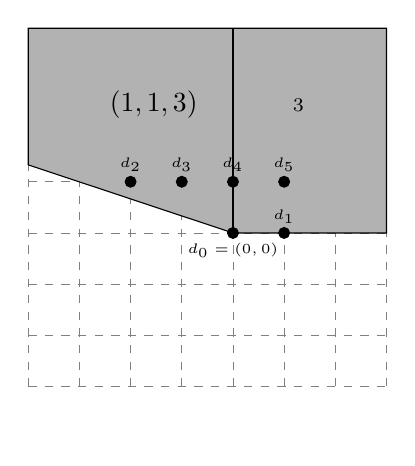
\begin{tikzpicture}[scale = .65]
\draw[step=1cm,gray,dashed,very thin] (0,0) grid (7,7);
\draw[fill=gray!60] (4,3)--(0,4.33)--(0,7)--(7,7)--(7,3)--(4,3);
\draw (4,3) -- (4,7);
\filldraw[black] (5,3) circle (3pt);
\filldraw[black] (5,3) circle (0pt) node[anchor=south]{\tiny $d_1$};
\filldraw[black] (3.5,5.5) circle (0pt) node[anchor=east]{{ $\PP(1,1,3)$}};
\filldraw[black] (4.8,5.5) circle (0pt) node[anchor=west]{{ $\cH_3$}};
\filldraw[black] (2,4) circle (3pt) node[anchor=south]{\tiny$d_2$};
\filldraw[black] (3,4) circle (3pt) node[anchor=south]{\tiny$d_3$};
\filldraw[black] (4,4) circle (3pt) node[anchor=south]{\tiny$d_4$};
\filldraw[black] (5,4) circle (3pt) node[anchor=south]{\tiny$d_5$};
\filldraw[black] (4,3) circle (3pt) node[anchor=north]{\tiny$d_0=(0,0)$};
\filldraw[black]  (1,-1) circle (0pt);
\end{tikzpicture}
\qquad
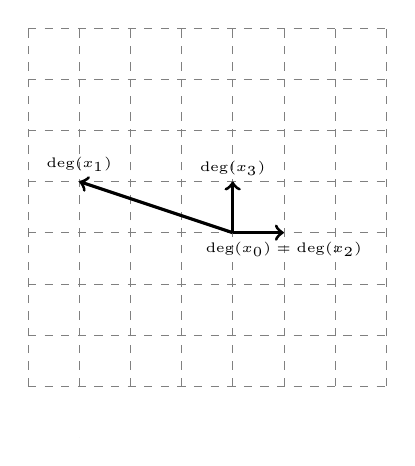
\begin{tikzpicture}[scale = .65]
\draw[step=1cm,gray,dashed,very thin] (0,0) grid (7,7);
\node[anchor=north] at (5,3){\tiny $\deg(x_0)=\deg(x_2)$};
\draw[black, ->, line width = .4mm] (4,3)--(5,3);
\draw[black, ->, line width = .4mm] (4,3)--(4,4);
\draw[black, ->, line width = .4mm] (4,3)--(1,4);
\node at (4,4.25){\tiny $\deg(x_3)$};
\node[anchor=south] at (1,4) {\tiny $\deg(x_1)$};
\filldraw[black]  (1,-1) circle (0pt);
\end{tikzpicture}
\qquad
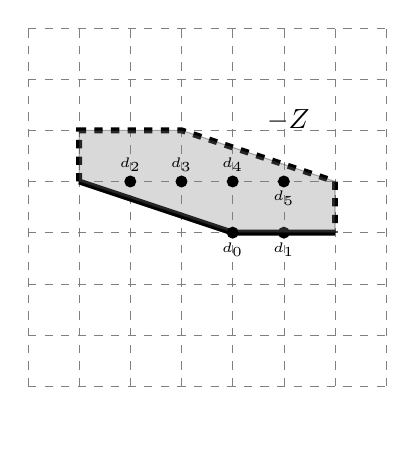
\begin{tikzpicture}[scale = .65]
\draw[step=1cm,gray,dashed,very thin] (0,0) grid (7,7);
\filldraw[black] (4.3,5.2) circle (0pt) node[anchor=west]{{ $- Z$}};
\filldraw[black] (5,3) circle (3pt) node[anchor=north]{\tiny $d_1$};
\draw[black, line width = .75mm] (6,3)--(4,3)--(1,4);
\draw[black, dashed, line width = .75mm] (1,4) -- (1,5)--(3,5)--(6,4)--(6,3);
\draw[fill = gray, opacity = .3] (4,3)--(1,4) -- (1,5)--(3,5)--(6,4)--(6,3)--(4,3);
\filldraw[black] (2,4) circle (3pt) node[anchor=south]{\tiny$d_2$};
\filldraw[black] (3,4) circle (3pt) node[anchor=south]{\tiny$d_3$};
\filldraw[black] (4,4) circle (3pt) node[anchor=south]{\tiny$d_4$};
\filldraw[black] (5,4) circle (3pt) node[anchor=north]{\tiny$d_5$};
\filldraw[black] (4,3) circle (3pt) node[anchor=north]{\tiny$d_0$};
\filldraw[black]  (1,-1) circle (0pt);
\end{tikzpicture}
\caption{The secondary fan for a Hirzebruch surface $\cH_3$ has two maximal
chambers: one corresponding to $\cH_3$ and the other to $\PP(1,1,3)$.  The
Bondal--Thomsen collection $\Theta$ consists of the degrees in a half-open
zonotope $Z$ determined by the degrees of the variables.   In this
example, $\Theta$ consists of the $6$ degrees $-d_i$, with $d_i$ as marked in
$-Z$.}
\label{fig:HirzSecondaryFan}
\end{figure}

\begin{example}\label{ex:hirzGKZ}
Let $X=\cH_3$ be a Hirzebruch surface of type $3$. As we have already seen, its secondary fan has two maximal chambers (see Figure~\ref{fig:HirzSecondaryFan}): one corresponding to $\cH_3$, and the other to the weighted projective stack $\PP(1,1,3)$.
After choosing $\tsX$ (see \cref{subsec:constructionOfWX}), $D_{\Cox}$ is generated by pullbacks of line bundles from $\cH_3$ and $\PP(1,1,3)$.
Some of these ``glue,'' for example, the pullbacks of $\cO_{\cH_3}(0,d)$ and $\cO_{\PP(1,1,3)}(3d)$ agree for all $d\in \ZZ$.  For other bundles, the correspondence is more subtle. For instance, the Fourier--Mukai transform of the structure sheaf of the exceptional curve on $\cH_3$ is supported on the stacky point of $\PP(1,1,3)$.

The Bondal--Thomsen collection corresponds to a set of degrees in $\Cl(\cH_3)= \ZZ^2$.  Each of these degrees has the form $-d_i$ where $d_i$ is some effective degree.  The secondary fan lives in $\Cl(\cH_3)\otimes_{\ZZ} \QQ$ and has support equal to the effective cone of $\cH_3$.  So we can overlay the secondary fan with the $d_i$ from the  Bondal--Thomsen collection.  This is illustrated in
Figure~\ref{fig:HirzSecondaryFan}.

To state Theorem~\ref{thm:main1} precisely, we need to assign to each element $-d\in \Theta$ an appropriate object in
$D_{\Cox}$. This issue is that we have too many possible choices!  For a given $-d$ should we take the pullback of $\cO_{\PP(1,1,3)}(-d)$ or the pullback of $\cO_{\cH_3}(-d)$.  If these always coincided, we would not have an issue, but we are not that lucky.

So for a given degree $d$, how do we decide when to pull back from $\PP(1,1,3)$ and when to pullback from $\cH_3$?  We let the secondary fan be our guide.  For instance, referring to Figure~\ref{fig:HirzSecondaryFan},
$d_5$ lies in the chamber for $\cH_3$; thus, we define $\cO_{\Cox}(-d_5)$ as
the pullback of $\cO_{\cH_3}(-d_5)$.

We thus pull back $-d_1$ and $-d_5$ from $\cH_3$, and $-d_2$ and $-d_3$ from $\PP(1,1,3)$; for $-d_0$ and $-d_4$, either choice will work because the pullbacks will coincide.
\end{example}
This example indicates the general recipe.
\begin{defn}\label{defn:ThetaCox}
Choose $-d \in \Theta$.  Since $d$ is an effective degree, its image in $\Cl(X)_\RR$ lies in one of the maximal chambers $\Gamma_i$ of the secondary fan, and this chamber corresponds to some $\sX_i$.  For this degree, we define $\cO_{\Cox}(-d)\ce\pi_i^*\cO_{\sX_i}(-d)$.
\end{defn}
We also need to choose an ordering on the elements of $\Theta$.
\begin{defn}\label{defn:ordering}
   The set $\Theta$ is equipped with a partial ordering such that $-d \le -d'$ if and only if $d - d'$ is effective. We choose any refinement of this partial ordering to a total ordering $-d_0, \dots, -d_t$.
\end{defn}

\begin{example}
Continuing with the notation of Figure~\ref{fig:HirzSecondaryFan}, the ordering would be $-d_5<-d_4<-d_3<-d_2<-d_1<-d_0$
\end{example}


%%%%%%%%%%%%%%%%%%%%%%%%%%%%%%%%%%%%%%%%%%%%%%%%%%%%%%%%%%%%%%%%%%%%%%%
\section{Lecture 13 (John Cobb): The Cox category, II: Fourier-Mukai Transforms}\label{lec:13-DCox-FM-transform}
\label{sec:FMTransform}
Each of the toric stacks $\sX_1, \dots, \sX_r$ contains a copy of the same dense torus.  In particular, there is a natural birational map $\sX_i\dashrightarrow \sX_j$ for any $i,j$.  We write $\Gamma_{ij}$ for the graph of this birational map as a subvariety of $\sX_i\times \sX_j$.  There are natural projection maps $p,q$ from $\sX_i\times \sX_j$ to the two factors. We obtain the following diagram:
\[
\xymatrix{
&\sX_i\times \sX_j\ar[ld]_{p}\ar[rd]^{q}&\\
\sX_i&&\sX_j.
}
\]
This allows us to define a Fourier--Mukai transform
\[
\Phi_{ij}\colon D^b(\sX_i)\to D^b(\sX_j) \text{ where } \Phi_{ij}(\cE) := Rq_*\left(p^*\cE \Lotimes_{\cO_{\sX_i\times \sX_j}} \cO_{\Gamma_{ij}}\right).
\]
At a more concrete level, the Fourier--Mukai transform can be understand as follows.  There is a Hanlon-Hicks-Lazarev complex $F$ which resolves $\Gamma_{ij}\subseteq \sX_i\times \sX_j$ and so we can ``underive'' the tensor product, by replacing $\cO_{\Gamma_{ij}}$ by $F$:
\[
\Phi_{ij}(\cE) = Rq_*\left(p^*\cE \otimes_{\cO_{\sX_i\times \sX_j}} F\right).
\]


This provides a geometric way to ``move'' a sheaf (or an object of the derived category) from one of the $\sX_i$ to all of the other.  Namely, imagine we have a sheaf $\cE_1$ on $\sX_1$.  For each $j$, we obtain $\Phi_{1j}(\cE_1)$ on $\sX_j$.  Since the $\sX_i$ all agree on the dense torus, $\Phi_{1j}(\cE_1)$ will agree with $\cE_1$ on the dense torus, and will only exhibit different behavior on the toric boundary.

\begin{example}
    For any $i,j$ we have $\Phi_{ij}(\cO_{\sX_i})=\cO_{\sX_j}$.  Why?  The pullback $p^*\cO_{\sX_i}$ is simply $\cO_{\sX_i\times \sX_j}$; this is a line bundle, and so the derived tensor product with $\cO_{\Gamma_{ij}}$ is simply the (underived) tensor product, which is
    \[
    \cO_{\sX_i\times\sX_j} \otimes_{\cO_{\sX_i\times \sX_j}}\cO_{\Gamma_{ij}} = \cO_{\Gamma_{ij}}.
    \]
We thus have that $\Phi_{ij}(\cO_{\sX_j})$ is the pushforward of $\cO_{\Gamma_{ij}}$ under the natural birational morphism $\Gamma_{ij}\to \sX_j$.  We then have $R(q|_{\Gamma_{ij}})_* \cO_{\Gamma_{ij}} = \cO_{\sX_j}$ by \cite{king}*{Proposition 3.5}.
\end{example}

\begin{example}
    If $i=j$ then $\Gamma_{ij}$ is simply the diagonal $\Delta\subseteq \sX_i\times \sX_i$.  In this case,  $\Phi_{ii}$ is a Fourier--Mukai transform with respect to a resolution of the diagonal.  Thus $\Phi_{ii}$ is equivalent to the identity functor.  See for example \daniel{Add reference to Caldararu notes}.
\end{example}

\begin{example}\label{ex:HirzFMTransform}
Let us return to our running example of the Hirzebruch surface of type $3$.  Consider
\[
\Phi_{21}\colon D(\mathcal H_3) \to D(\PP(1,1,3)).
\]
Let us consider what happens when we apply this nontrivial transform to the Bondal--Thomsen element $\cO_{\mathcal H_3}(-1,0)$.  To perform the computation, we start with the Hanlon-Hicks-Lazarev resolution for $\Gamma_{ij}$.  This has the form
\[
\begin{matrix}
    \cO(0,0,0)\\
    \oplus \\
    \cO(2,-1,-2)\\
    \oplus\\
    \cO(1,-1,-1)
\end{matrix}
\longleftarrow
\begin{matrix}
    \cO(1,-1,-2)^2\\
    \oplus \\
    \cO(2,-1,-3)^2\\
    \oplus\\
    \cO(0,-1,-1)^2 \\
    \oplus \\
    \cO(-1,0,-1)
\end{matrix}
\longleftarrow
\begin{matrix}
    \cO(1,-1,-3)\\
    \oplus \\
    \cO(2,-1,-4)\\
    \oplus\\
    \cO(0,-1,-2)\\
    \oplus \\
    \cO(-1,-1,-1)
\end{matrix}.
\]
Note that each line bundle is a box product from the factors.  For instance, $\cO(2,-1,-2)$ means $\cO_{\mathcal H_3}(2,-1) \boxtimes \cO_{\PP(1,1,3)}(-2)$.

When we pull back $\cO_{\mathcal H_3}(-1,0)$ and tensor with this complex, we get:
\[
\begin{matrix}
    \cO(-1,0,0)\\
    \oplus \\
    \cO(1,-1,-2)\\
    \oplus\\
    \cO(0,-1,-1)
\end{matrix}
\longleftarrow
\begin{matrix}
    \cO(0,-1,-2)^2\\
    \oplus \\
    \cO(1,-1,-3)^2\\
    \oplus\\
    \cO(-1,-1,-1)^2 \\
    \oplus \\
    \cO(-2,0,-1)
\end{matrix}
\longleftarrow
\begin{matrix}
    \cO(0,-1,-3)\\
    \oplus \\
    \cO(1,-1,-4)\\
    \oplus\\
    \cO(-1,-1,-2)\\
    \oplus \\
    \cO(-2,-1,-1)
\end{matrix}.
\]
Since each of the terms is box product, we can thus compute the pushforward of this complex in terms of the pushforwards of the terms.  For a box product $\cF\boxtimes \cG$ on a product $X_1\times X_2$, the projection formula implies that
\[
R\pi_{1*}\left(\cF\boxtimes \cG\right) \cong \cF \otimes R\pi_{1*}(\cG).
\]
 This allows us to easily compute the pushforward of each term.  For instance:
\[
Rp_*(\cO(1,-1,-2)) = Rp_*\left((\cO_{\mathcal H_3})(1,-1)\boxtimes \cO_{\PP(1,1,3)}(-2)\right) = H^*(\cO_{\mathcal H_3}(1,-1)) \otimes \cO_{\PP(1,1,3)}(-2))
\]
which equals $0$ because $\cO_{\mathcal H_3)}(1,-1)$ has no cohomology whatsoever by Corollary~\ref{cor:BTNoCohom}.    In fact, in this example, all of the terms vanish except $\cO(-2,0,-1)$ which has nonzero $H^1$ and so we end up with
\[
\Phi_{21}(\cO_{\mathcal H_3}(-1,0)) \cong H^1(\mathcal H_3, \cO(-2,0)) \otimes \cO_{\PP(1,1,3)}(-1) \cong \cO_{\PP(1,1,3)}(-1).
\]
% Degrees:
% --conversion to P(1,1,3) is a+3b
% %0,0,0,0
% %2,-1,1,-1
% %1,-1,2,-1
% 0,0,0
% 2,-1,-2
% 1,-1,-1

% 1,-1,-2 (2)
% 2,-1,-3 (2)
% 0,-1,-1 (2)
% 0,-1,-3


% %1,-1,0,-1
% %2,-1,-1,-1
% %0,-1,1,-1
% %-1,-1,2,-1

% \cO(1,-1,-3) \\
% \oplus \\
% \cO(2,-1,-4) \\
% \oplus \\
% \cO(0,-1,-2) \\
% \oplus \\
% \cO(0,-1,-1) \\


\end{example}


\begin{remark}
    There is also an algebraic method to ``move'' a sheaf from one of the $\sX_i$ to all of the other.
    %Namely, if we choose a graded $S$-module $M$ such that $M|_{\sX_1}\cong \cE_1$ then we can obtain sheaves $M|_{\sX_j}$ on each of the $\sX_j$.  But there is an issue with this process:  the sheaf $M|_{\sX_j}$ may depend not just on $\cE_1$ but also on the choice of the module $M$.
 For instance, as in Example~\ref{ex:HirzFMTransform}, let us start with $\cO_{\cH_3}(-1,0)$ on $\cH_3$.  We can represent this by a graded $S$-module: for instance $S(-1,0)$ is a natural choice, as $S(-1,0)|_{\cH_3} = \cO_{\cH_3}(-1,0)$.  We can then use $S(-1,0)$ to determine a sheaf on $\PP(1,1,3)$ namely: $S(-1,0)|_{\PP(1,1,3)} = \cO_{\PP(1,1,3)}(-1)$.

 But one should be cautious, as the outcome of this method depends on the module one uses to represent the initial sheaf.  For instance, we could also have represented $\cO_{\cH_3}(-1,0)$ via a different module.  A rather artificial choice would be to write $M=S(-1,0) \oplus S/(x_0,x_2)$.  Since $(x_0,x_2)$ is a component of the irrelevant ideal for $\cH_3$, we have $(S/(x_0,x_2))|_{\cH_3}=0$ as a sheaf on $\cH_3$.  Thus $M|_{\cH_3} \cong \cO_{\cH_3}(-1,0)$.  But on $\PP(1,1,3)$, $(x_0,x_2)$ is not a component of the irrelevant ideal.  It is the ideal of the singular point  $p=[0:0:1]$.  Thus $M|_{\PP(1,1,3)} = \cO_{\PP(1,1,3)}(-1) \oplus \cO_p$.


% Then we have $M|_{\cH_3} = \cO_{\cH_3}(-1,0)$ and $M|_{\PP(1,1,3)}=\cO_{\PP(1,1,3)}(-1)$.

%  $I=\langle x_0,x_2\rangle$.  We have  $I(1,0)|_{\cH_3}=\cO_{\cH_3}$ but of course $S|_{\cH_3}=\cO_{\cH_3}$ as well.  The corresponding sheaves on $\PP(1,1,3)$ are distinct however:  $S|_{\PP(1,1,3)}=\cO_{\PP(1,1,3)}$ whereas $I(1,0)|_{\PP(1,1,3)}$
\end{remark}


\begin{remark}\label{rmk:WhatIsRevisedKingsConjectureAbout}
What does the Revised King's Conjecture really tell us?  Let's first address what it specifically tells us about sheaves and multigraded rings.

We get a uniqueness property akin to Theorem~\ref{thm:UniquenessAndFSEC}.  Namely, take a sheaf $\cE$ on a toric variety $X$.  Because $\Theta$ generates $D(X)$, one can represent $\cE$ in terms of the Bondal--Thomsen collection, but this representation will often be fundamentally non-unique.  However, if we want to represent $\cE$ AND the Fourier--Mukai transforms of $\cE$ to the other $\sX_i$ from the secondary fan, then we can do this in a unique (up to homotopy) way.  This is the statement of Corollary \daniel{FILL IN}.  In short: in some sense, it is simpler to classify sheaves on the whole secondary fan, than it is to just classify sheaves on a single toric variety $X$.

So the theorem tells us that while King's Conjecture was false, the underlying idea was very much correct.  The cases where full strong exceptional cases of line bundles exist--projective space, products, projective bundles, etc--are indicative of what happens in the general case.  The correct statement just required a framework that was not yet obvious back then.
\end{remark}
